% =====================================================================
%  Junior Independent Work: Prospectus Draft
%  Steven Goetz, Princeton Economics.  Adviser: Pablo Zarate
%  12-page limit excludes the title page and the bibliography.
%  Every number comes from Part 4 of the "JIW Database" Colab notebook.
% =====================================================================
\documentclass[12pt]{article}

\usepackage[margin=1in]{geometry}
\usepackage{setspace}
\usepackage{booktabs}
\usepackage{adjustbox}
\usepackage{graphicx}
\usepackage{float}
\usepackage{etoolbox}
\AtBeginEnvironment{table}{\singlespacing}
\AtBeginEnvironment{figure}{\singlespacing}
\usepackage{amsmath}
\usepackage{pgfplots}
\pgfplotsset{compat=1.17}
\usepgfplotslibrary{groupplots}
\usepackage[hidelinks]{hyperref}
\usepackage{natbib}
\bibliographystyle{apalike}
\usepackage{titlesec}
\titlespacing*{\section}{0pt}{8pt}{2pt}
\titlespacing*{\subsection}{0pt}{6pt}{1pt}
\titlespacing*{\paragraph}{0pt}{3pt}{1em}
\setlength{\textfloatsep}{10pt}
\setlength{\intextsep}{8pt}

\begin{document}

% ------------------------- Title page (not counted) -------------------
\begin{titlepage}
\centering
\vspace*{1.6in}
{\LARGE Buying Time, Missing the Signs:\\[6pt] Cause of Distress and Lender Response in Liability Management\par}
\vspace{0.6in}
{\large Junior Independent Work Prospectus\par}
\vspace{0.6in}
{\large Steven Goetz\par}
\vspace{0.15in}
{\large Advisers: Professor Smita Brunnermeier and Pablo Zarate\par}
\vspace{0.15in}
{\large Department of Economics, Princeton University\par}
\vspace{0.15in}
{\large \today\par}
\vfill
\begin{minipage}{0.85\textwidth}
\centering
\emph{This paper represents my own work in accordance with University regulations.}\\[10pt]
/s/ Steven Goetz
\end{minipage}
\vspace{0.8in}
\end{titlepage}

\setcounter{page}{1}
\doublespacing

% ---------------------------------------------------------------------
\section{Introduction}
% ---------------------------------------------------------------------

When a company cannot pay its debts it can restructure in bankruptcy court or negotiate with its creditors outside it. Over the past decade the out-of-court route has taken a new form, the liability management exercise (LME): the borrower and a majority of its lenders rewrite the debt, usually extending maturities and adding new senior loans, and the firm avoids Chapter 11 for now \citep{buccolanini2024}. Supporters say the deal buys the firm ``runway'' to recover. The first systematic evidence says otherwise \citep{roerotaru2026}. In my coding of the LMEs in that study, 79\% of those old enough to judge ended in Chapter 11 bankruptcy or a second restructuring within two years.

Two kinds of deal appear in this paper, and the difference matters throughout. In a \emph{pro rata} exchange every lender in a class of debt is offered the same trade. In a \emph{non-pro rata} LME the borrower and a majority of its lenders amend the loan contract so that the participating lenders move ahead of the others in the line for repayment \citep{roerotaru2026}. The deal is called \emph{coercive} because a lender who declines is left with a weaker claim \citep{buccolakahan2025}. Many of these borrowers are owned by private equity firms, or \emph{sponsors}, whose equity is worth something only while the firm stays out of bankruptcy \citep{buccola2023}. Exchanges of both kinds are common. Together they were half of the 548 U.S.\ corporate defaults that S\&P recorded from 2018 to 2025 \citep{spdefault}.

That evidence treats every distressed firm as the same kind of patient. Consider a cruise line in 2020, whose customers disappeared for a year, and a floppy disk manufacturer, whose customers are never coming back. Both may be unable to pay their debts and both may sign the same deal, but time can only help the first. Corporate finance has long drawn this line between \emph{financial} distress, a sound business with too much debt, and \emph{economic} distress, a business that has lost its value \citep{wruck1990, andrade1998}. It has not been applied to modern exchanges.

This paper asks two questions. First, does the outcome of a distressed exchange depend on the cause of the borrower's distress, a temporary shock versus a structural decline of the business? Second, do the lenders whose consent the exchange requires write different terms depending on that cause?

The questions matter because the alternative to an exchange is costly \citep{antill2026} and the exchange is not free \citep{elkamhi2024}. A firm that restructures out of court and then fails pays for distress twice. The policy debate is whether courts and contracts should restrain these deals \citep{ellias2020, buccolakahan2025}. If they fail mainly for one identifiable kind of firm, the remedy is better screening of who gets one, not a ban.

The contribution is threefold. I build a continuous measure of the cause of distress for 275 U.S.\ exchanges from rating-agency text published before each deal. I use it to give what is, to my knowledge, the first estimate of post-exchange outcomes conditional on cause. And I observe the terms lenders accept at the exchange itself, where prior work observes their response in the contracts of new loans \citep{buccolanini2024, badawi2024, ivashina2025}. The design describes for which firms failure follows an exchange. It does not identify whether the exchange beat Chapter 11 for a given firm. The data are already assembled.

% ---------------------------------------------------------------------
\section{Literature Review}
% ---------------------------------------------------------------------

Whether an out-of-court exchange is worth doing depends on what it costs relative to bankruptcy, on who is pushing for it, and on whether lenders can tell which borrowers will use the time well. Prior work studies each of these in isolation. None of it asks whether the answer depends on why the firm is distressed, which an older literature on classifying distress gives me the tools to measure.

\emph{Outcomes.} Whether an exchange is worth doing depends on what it avoids. \citet{antill2026} show experimentally that learning of a Chapter 11 filing cuts consumers' willingness to pay by 17--28\%, a cost that arrives only at the filing. But \citet{elkamhi2024} estimate that roughly 64\% of distress costs accrue \emph{before} default. The two findings measure different costs at different moments, so an exchange avoids the first and prolongs the second, and it pays only if it ends the distress. \citet{roerotaru2026} find that coercive LMEs usually do not. \citet{harmon2026} reaches a similar conclusion from trading prices, but on 16 deals, which is consistent with their result rather than independent confirmation of it. Both studies pool firms.

\emph{Incentives.} \citet{ellias2020} attribute aggressive restructurings to weakened fiduciary duties, which leave the equity of an insolvent firm as an option that costs its holders nothing to keep alive. \citet{buccola2023} attributes them to private equity sponsors who gain from postponing losses. These papers explain why borrowers \emph{propose} exchanges. They do not imply that every distressed firm \emph{completes} one, since lenders must agree and many firms file instead. \citet{gilson1990} found that only about half of the distressed firms that attempted a private restructuring completed one. That selection is a central issue for my design (Section~\ref{sec:method}).

\emph{Lender responses.} \citet{buccolanini2024} show loan contracts added protections after one landmark deal but not another. \citet{badawi2024} find those protections were not reflected in loan prices, while \citet{ivashina2025} find prices respond to contract weakness only coarsely. All three study the terms of \emph{new} loans. None observes what lenders demand when a distressed borrower asks for an exchange, by which point the rating agencies have published why the firm is distressed. \citet{kahl2002} predicts lenders who cannot yet tell which kind of distress they face will rationally grant short extensions and learn. The closest precedent is older: \citet{asquith1994} find that banks facing distressed junk-bond issuers rarely forgave principal and instead deferred payments.

\emph{Classifying distress.} \citet{andrade1998} find distress costs are negligible for firms whose operating margins held up and 10--20\% of value for firms whose business also declined. \citet{asquith1994} separate industry, firm-specific and leverage causes. \citet{denis1995}, lacking financial statements, code causes from news text. The underlying mechanism is debt overhang \citep{myers1977}: relieving the debt of a sound firm restores its incentive to invest, while no debt contract restores a lost market. This literature studies the leveraged buyouts of the 1980s. It has not been applied to modern exchanges, which is the gap this paper fills. 


% ---------------------------------------------------------------------
\section{Data}
% ---------------------------------------------------------------------

\paragraph{Sample.} The unit of observation is a distressed exchange by a U.S.\ company. I combine two sources. The first is the list of 89 coercive, non-pro rata LMEs from 2014--2025 hand-collected by \citet{roerotaru2026}. The second is S\&P's annual default studies for 2018--2025 \citep{spdefault}, which list every rated issuer that defaulted and the reason. They record 548 U.S.\ defaults, of which 275 are tagged as distressed exchanges, meaning creditors received less than promised and the firm would otherwise have defaulted. I drop 12 that were not U.S.\ operating companies or were mis-tagged bankruptcies, and set aside 75 that were either already in the LME list or other exchanges by the same companies. The remaining 188 are \emph{pro rata} exchanges, in which all holders of a debt class are treated alike. The sample is therefore 277 deals: 89 LMEs and 188 pro rata exchanges.

Fifty-four of the 89 LMEs also appear in S\&P's tables. Most of the other 35 added new senior debt without impairing existing claims, which S\&P does not count as a default. The 188 pro rata exchanges are new to this literature as a group studied in its own right. S\&P covers only publicly rated issuers, so unrated borrowers are not observed.

\paragraph{Outcome.} A deal \emph{fails} if the firm files for bankruptcy or completes another distressed exchange. I measure failure within one, two and three years, using the LME study's coding for LMEs and S\&P's later default records, checked against court dockets, for pro rata deals. A deal enters the $h$-year sample only if it closed at least $h$ years before the data cutoff of 14 January 2026, so recent deals are not counted as survivors merely because they are young. Failure therefore combines two events. I also report them separately, because a second exchange can be a planned next step rather than a breakdown \citep{kahl2002}.

\paragraph{Cause of distress.} For each deal I collect the S\&P and Moody's rating-action text from the twelve months before it, together with the agencies' description of the two-year earnings trend. A written codebook assigns one of three labels: shock (a temporary demand or financial shock to an intact business), structural (secular industry decline, firm-specific deterioration, or a legal or regulatory blow), or mixed. The rules are fixed in advance and code the driver the agency \emph{names}, not its outlook for the firm. A temporary shock is still an operating problem, so the labels are not financial against economic distress. They capture how persistent the agencies judge the operating damage to be, which is the dimension on which runway should matter.

The mixed label is a judgment call, so the main measure is continuous rather than the labels themselves. Each deal is coded 70 times by three OpenAI language models (30 runs each of two smaller models and 10 of a larger one) that see only the pre-deal text and the codebook, never the deal type or the outcome. The \emph{structural score} is the share of those codings that are structural, counting a mixed coding as one half. It runs from 0 (every coding says shock) to 1 (every coding says structural). Two deals have no agency text, leaving 275 scored deals (87 LMEs and 188 pro rata).

Revlon in 2020 shows the middle of the scale. Its rating text names the pandemic on top of years of declining sales, and the coders split (score 0.51).

\paragraph{Terms.} For the 242 exchanges S\&P records, I code what lenders gave and got from the agencies' default releases. The terms fall into three groups. \emph{Balance-sheet repair} reduces what the firm owes: a \emph{haircut} (principal is written down) or conversion of debt into equity. \emph{Lender control} gives creditors power over the firm: a controlling equity stake, board rights, tighter \emph{covenants} (contract limits on what the borrower may do), or new loans that rank ahead of existing debt. \emph{Runway} gives time without reducing debt: a maturity extension, or \emph{payment-in-kind} (PIK) interest, paid in more debt instead of cash. Forty of the pro rata deals and two LMEs are open-market repurchases, in which the firm buys back its own debt below face value from willing sellers. They carry no negotiated terms, so the terms analysis uses the other 200 exchanges, 148 of them pro rata.

\begin{table}[H]
\centering
\caption{Summary statistics}
\label{tab:sumstats}
\small
\begin{adjustbox}{max width=\textwidth}
\begin{tabular}{l r r r}
\toprule
 & Pro rata exchanges & LMEs & All \\
\midrule
Deals & 188 & 87 & 275 \\
\addlinespace \textit{Structural score (0 = shock, 1 = structural)} & & & \\
\quad Mean & 0.66 & 0.73 & 0.69 \\
\quad Standard deviation & 0.43 & 0.38 & 0.42 \\
\quad Share low (0--0.33) & 31\% & 23\% & 28\% \\
\quad Share middle (0.33--0.67) & 6\% & 9\% & 7\% \\
\quad Share high (0.67--1) & 63\% & 68\% & 64\% \\
\quad Share structural, binary (score above one half) & 67\% & 72\% & 69\% \\
\addlinespace \textit{Original three labels} & & & \\
\quad Share shock & 26\% & 17\% & 23\% \\
\quad Share mixed & 27\% & 36\% & 30\% \\
\quad Share structural & 47\% & 47\% & 47\% \\
\addlinespace \textit{S\&P rating one year before the deal (15 = B$-$, 16 = CCC+)} & & & \\
\quad Mean notch & 15.35 & 15.22 & 15.32 \\
\quad Standard deviation & 1.39 & 1.03 & 1.32 \\
\quad Deals with a rating & 142 & 37 & 179 \\
\addlinespace \textit{Timing} & & & \\
\quad Share closed in 2020 & 21\% & 10\% & 18\% \\
\addlinespace \textit{Outcomes (among deals observed for the full horizon)} & & & \\
\quad Deals observable at 2 years & 141 & 43 & 184 \\
\quad\quad Failed again within 2 years & 40\% & 79\% & 49\% \\
\quad\quad Filed for bankruptcy within 2 years & 16\% & 40\% & 22\% \\
\quad Deals observable at 3 years & 106 & 28 & 134 \\
\quad\quad Failed again within 3 years & 51\% & 86\% & 58\% \\
\bottomrule
\end{tabular}
\end{adjustbox}
\begin{minipage}{0.9\textwidth}\vspace{4pt}\footnotesize
\textit{Notes.} The 275 deals with a structural score (two deals with no pre-deal agency text are excluded). Failure is a Chapter 11 filing or a further distressed exchange. Ratings are available for S\&P-rated issuers only.
\end{minipage}
\end{table}


Table~\ref{tab:sumstats} summarises the data. The score is bimodal: 60\% of deals lie in the top third and 26\% in the bottom third. Failure is common, 40\% of pro rata exchanges and 79\% of LMEs within two years, so the outcome has ample variation.

Three features of the measure bear on its credibility. First, agreement among coders is high: the three models' scores correlate 0.84--0.86 with one another and the intraclass correlation of their average is 0.94 \citep{koo2016}. Second, the models were trained after many of these outcomes were known, so they might be recalling which firms failed. Re-coding with company names removed barely changes the score (correlation 0.95) or the estimate from that model (0.16 against 0.18). Third, the quotations each coder reads were selected in a first pass by a language-model assistant, so the agreement is an upper bound. A human-coded subsample from the full rating reports addresses this (Section~\ref{sec:next}).

% ---------------------------------------------------------------------
\section{Methodology}
\label{sec:method}
% ---------------------------------------------------------------------

\paragraph{Hypotheses.} \emph{H1 (outcomes):} failure after an exchange rises with the structural score, $\beta > 0$ in equation~\eqref{eq:main}. Debt overhang theory predicts that an exchange can cure a sound firm with too much debt but not a declining business. H1 is rejected if $\beta$ is zero or negative, or if it disappears once the firm's prior rating is held fixed, which would mean the score only restates default risk. \emph{H2 (screening):} lenders who act on the diagnosis give high-score borrowers more lender control and less pure runway. For balance-sheet repair the prediction is two-sided. Overhang theory says a debt cut helps the sound firm most, while a lender facing a declining firm may prefer equity to an extension. The null is that terms follow the form and year of the deal and not the diagnosis.

\paragraph{Specification.} For H1 I estimate a linear probability model on deals observed for at least $h$ years,
\begin{equation}
\text{Fail}_{i,h} = \alpha + \beta\,\text{Score}_i + \gamma_{t(i)} + \delta_{j(i)} + \varepsilon_i ,
\label{eq:main}
\end{equation}
where $\gamma_t$ and $\delta_j$ are deal-year and industry fixed effects (S\&P's eleven industry groups) and standard errors are clustered by issuer, since some firms exchange more than once. $\beta$ is the difference in failure probability between a firm every coder calls structural and one every coder calls shock, in the same year and industry. The fixed effects matter because shocks cluster in 2020 and structural decline clusters in a few industries. They explain a fifth of the variation in the score, so most of what identifies $\beta$ is variation within a year and an industry. I estimate the model for pro rata exchanges, where deal form is held fixed, and then pool with an LME indicator, which asks whether deal form matters once cause is held fixed. For H2 the dependent variable is each term in turn. Because that is many tests, the single pre-specified test is a strictness index, the average of the standardised terms signed so that higher is tougher on the borrower \citep{kling2007}.

The data are a cross-section of deals, not a panel, and $\beta$ is not the effect of an exchange. Structural firms may fail more with or without one, and I have no firm-level counterfactual. $\beta$ measures for which firms failure follows an exchange, which is what a lender asked to grant one needs to know. Four threats to reading it as the effect of cause follow, with the planned response to each.

\paragraph{Selection into exchange.} Borrowers may always want an exchange, but lenders must agree, and half of the defaults in the S\&P universe were bankruptcies or missed payments instead. If lenders refuse the least viable structural firms, those in my sample are the better ones and $\beta$ is biased toward zero. If only desperate shock firms exchange, the bias runs the other way. I will score the 273 non-exchange defaults in the same S\&P studies and compare firms that exchanged with firms that filed directly. This signs the bias but does not remove it.

\paragraph{Measurement.} Rating analysts write knowing how weak the firm is, so a ``structural'' label could be a forecast of failure in other words. I address this in two ways. The score should be unrelated to the firm's rating a year before the deal, which is the agency's own summary of default risk, and I control for that rating. The rating is a coarse control, since most firms sit within two rating steps of each other, so this check can reject a strong forecast channel but not a weak one. And for the roughly one third of issuers with public financial statements, I will check the score against the operating-margin test of \citet{andrade1998}. That validation cannot cover private issuers, which is a limit of the design.

\paragraph{Vintage.} Shock-driven distress clusters in 2020, and credit conditions differ by year. Year fixed effects absorb common shocks, and I report $\beta$ separately by vintage and with 2020 excluded. The firms hit in 2020 were also helped by an unusually fast reopening of credit markets, so I put more weight on the by-vintage estimates than on the pooled one.

\paragraph{Functional form and power.} Equation~\eqref{eq:main} assumes failure is linear in the score. I test this with three bins of the score and a quadratic term. With 141 pro rata deals observable at two years, the smallest effect detectable with 80\% power is about 31 percentage points, which is larger than the preliminary estimate in Section~\ref{sec:results}. A significant estimate in a sample this size tends to overstate the truth, and insignificant results will be reported as imprecise rather than as zeros. For H2 the smallest detectable shift in the strictness index is 0.34, two thirds of its standard deviation, so the test can rule out strong screening but not mild screening.

% ---------------------------------------------------------------------
\section{Preliminary and Expected Results}
\label{sec:results}
% ---------------------------------------------------------------------

\paragraph{H1.} Figure~\ref{fig:bins} and Table~\ref{tab:reg_part1} report preliminary estimates. After a pro rata exchange, moving from a score of 0 to 1 raises two-year failure by 25 percentage points ($p = 0.02$; 95\% confidence interval 3 to 46). The binary version gives 20 points, and under the original three labels structural deals fail 36 points more often than shock deals (panels B and C). LMEs fail more often at every score, by 29 points in the pooled model and by 28 when I keep only the LMEs that S\&P also records as defaults.

\begin{figure}[H]
\centering
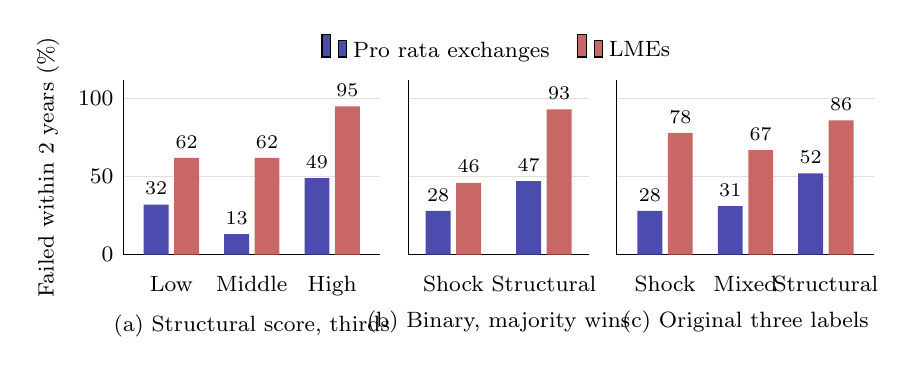
\begin{tikzpicture}
\begin{groupplot}[group style={group size=3 by 1, horizontal sep=10pt, yticklabels at=edge left, ylabels at=edge left},
  ybar, /pgf/bar width=9pt, height=3.8cm, ymin=0, ymax=112, ytick={0,50,100},
  ylabel={Failed within 2 years (\%)}, ylabel style={font=\footnotesize}, xtick=data,
  ticklabel style={font=\footnotesize}, xlabel style={font=\footnotesize}, enlarge x limits=0.3,
  nodes near coords, nodes near coords style={font=\scriptsize},
  ymajorgrids, grid style={gray!25}, axis lines*=left, tick style={draw=none}]
\nextgroupplot[width=0.40\textwidth, symbolic x coords={Low,Middle,High}, xlabel={(a) Structural score, thirds}]
\addplot[fill=blue!55!black!70, draw=none] coordinates {(Low,32) (Middle,13) (High,49)};
\addplot[fill=red!65!black!60, draw=none] coordinates {(Low,62) (Middle,62) (High,95)};
\nextgroupplot[width=0.32\textwidth, symbolic x coords={Shock,Structural}, xlabel={(b) Binary, majority wins}, enlarge x limits=0.5,
  legend style={at={(0.5,1.04)}, anchor=south, draw=none, font=\footnotesize, legend columns=2, /tikz/every even column/.append style={column sep=8pt}}]
\addplot[fill=blue!55!black!70, draw=none] coordinates {(Shock,28) (Structural,47)};
\addplot[fill=red!65!black!60, draw=none] coordinates {(Shock,46) (Structural,93)};
\legend{Pro rata exchanges, LMEs}
\nextgroupplot[width=0.40\textwidth, symbolic x coords={Shock,Mixed,Structural}, xlabel={(c) Original three labels}]
\addplot[fill=blue!55!black!70, draw=none] coordinates {(Shock,28) (Mixed,31) (Structural,52)};
\addplot[fill=red!65!black!60, draw=none] coordinates {(Shock,78) (Mixed,67) (Structural,86)};
\end{groupplot}
\end{tikzpicture}
\caption{Two-year failure rate by cause of distress and deal form}
\label{fig:bins}
\begin{minipage}{0.95\textwidth}\vspace{2pt}\footnotesize
\textit{Notes.} Deals observed for two years. Pro rata $n$: (a) 44,~15,~82; (b) 54,~87; (c) 36,~42,~63. LME $n$: (a) 8,~13,~22; (b) 13,~30; (c) 9,~12,~22.
\end{minipage}
\end{figure}

Table~\ref{tab:robust} varies the measure and the sample. The estimate is positive in every row, from 0.16 to 0.35, though not always significant. It is not explained by prior credit quality. The score is only weakly related to the rating a year earlier ($\rho = -0.11$, $p = 0.18$), and controlling for that rating gives 0.31. Without the open-market repurchases it is 0.21 ($p = 0.07$).

\begin{table}[H]
\centering
\caption{Cause of distress and post-exchange failure, three versions of the measure}
\label{tab:reg_part1}
\small
\begin{tabular}{l c c c c}
\toprule
 & Fail 2y & Fail 3y & Bankrupt 2y & Fail 2y (pooled) \\
 & (1) & (2) & (3) & (4) \\
\midrule
\multicolumn{5}{l}{\textit{Panel A: structural score (main)}} \\
\quad Structural score (0--1) & 0.215$^{**}$ & 0.162 & 0.105 & 0.233$^{***}$ \\
 & (0.092) & (0.130) & (0.069) & (0.082) \\
\quad LME &  &  &  & 0.274$^{**}$ \\
 &  &  &  & (0.117) \\
\multicolumn{5}{l}{\textit{Panel B: binary, majority wins (score above one half)}} \\
\quad Structural majority & 0.154$^{*}$ & 0.096 & 0.080 & 0.156$^{**}$ \\
 & (0.085) & (0.117) & (0.059) & (0.072) \\
\quad LME &  &  &  & 0.285$^{**}$ \\
 &  &  &  & (0.119) \\
\multicolumn{5}{l}{\textit{Panel C: original three labels (shock omitted)}} \\
\quad Mixed & 0.125 & $-0.073$ & 0.061 & 0.059 \\
 & (0.107) & (0.148) & (0.076) & (0.093) \\
\quad Structural & 0.362$^{***}$ & 0.393$^{**}$ & 0.210$^{**}$ & 0.234$^{**}$ \\
 & (0.113) & (0.164) & (0.086) & (0.094) \\
\quad LME &  &  &  & 0.301$^{***}$ \\
 &  &  &  & (0.117) \\
\midrule
Sample & Pro rata & Pro rata & Pro rata & All \\
Observations & 141 & 106 & 141 & 184 \\
\bottomrule
\end{tabular}
\begin{minipage}{0.95\textwidth}\vspace{4pt}\footnotesize
\textit{Notes.} Linear probability models; each panel is a separate set of regressions, all with year and industry fixed effects. Standard errors clustered by issuer in parentheses. $^{*}$p$<$0.1; $^{**}$p$<$0.05; $^{***}$p$<$0.01.
\end{minipage}
\end{table}


\begin{table}[H]
\centering
\caption{The structural score under alternative constructions}
\label{tab:robust}
\small
\begin{adjustbox}{max width=\textwidth}
\begin{tabular}{l r r r r}
\toprule
Specification & Coefficient & Std.\ error & $p$ & $n$ \\
\midrule
Main: structural score & 0.215$^{**}$ & 0.092 & 0.020 & 141 \\
\addlinespace
Earlier score from codings that allowed ``mixed'' & 0.248$^{**}$ & 0.109 & 0.023 & 141 \\
\addlinespace
First exchange per issuer only & 0.246$^{**}$ & 0.117 & 0.035 & 108 \\
Excluding open-market repurchases & 0.218$^{**}$ & 0.105 & 0.038 & 107 \\
Controlling for rating one year before the deal & 0.245$^{**}$ & 0.108 & 0.023 & 124 \\
\bottomrule
\end{tabular}
\end{adjustbox}
\begin{minipage}{0.95\textwidth}\vspace{4pt}\footnotesize
\textit{Notes.} Dependent variable: failure within two years of a pro rata exchange. Each row is a separate linear probability model with year and industry fixed effects unless stated, standard errors clustered by issuer; the coefficient shown is on the cause measure named in the row. $^{*}$p$<$0.1; $^{**}$p$<$0.05; $^{***}$p$<$0.01.
\end{minipage}
\end{table}


Three results temper this. First, the estimate is not significant at three years, and the two parts of failure share it about equally: 0.13 for bankruptcy ($p = 0.11$) and 0.12 for a repeat exchange with no bankruptcy ($p = 0.21$). If a second exchange is a planned step, as in \citet{kahl2002}, only the first half is failure. Second, the relationship is not cleanly linear. The 15 deals in the middle of the scale failed least (13\%), though a quadratic term is not significant and the group is too small to interpret. Third, the gradient is concentrated in the 2020 and 2021--22 deals (0.31 and 0.47). It is small in 2018--19 (0.13) and absent in the 35 deals from 2023 (39\% against 40\%). I still expect a positive final estimate, because the mechanism has theory and earlier evidence behind it, but the 2023 result means H1 could fail as later deals mature.

I see two readings of the 2023 result, and they predict different things. The shock behind that vintage was the 2022--23 rise in interest rates on floating-rate loans, which is a problem of leverage more than of operations and did not reverse the way a lockdown did. If that is right, the gradient should return once I code rate-driven distress separately. The second reading is timing: failures often arrive after two years, so the gradient should appear at three.


\paragraph{H2.} Table~\ref{tab:h2} reports the tests, and the preliminary results favour the null. The strictness index rises by 0.09 across the score ($p = 0.46$). Of the lender-control terms only covenant tightening moves ($+0.25$, $p = 0.06$), and one marginal result in nine is about what chance would produce. Pure runway is no less common for high-score borrowers ($-0.07$, $p = 0.56$). These are imprecise nulls and not zeros, because mild screening would go undetected.

I expect the null to hold, for two reasons. Loan terms have been found to spread by convention rather than by pricing \citep{badawi2024}, and the lenders who design an exchange are negotiating mainly over their position against other creditors, which depends on the contract and not on why the firm is distressed. If H2 is instead supported in the final data, the reading changes: lenders do screen, and the high failure rate of structural firms is a risk they priced. Terms do matter for outcomes: deals that cut debt fail at 29\% against 51\% for deals that only extend it.

\paragraph{Pitfalls.} A null on H2 cannot by itself separate lenders who fail to screen from lenders who, as in \citet{kahl2002}, knowingly grant a short extension and wait. Terms are coded from agency releases that describe covenants inconsistently, which biases H2 toward a null. Sponsor ownership, which the incentive literature stresses, is recorded for the LMEs but not yet for the pro rata deals.

\begin{table}[H]
\centering
\caption{Exchange terms and the structural score (H2)}
\label{tab:h2}
\small
\begin{tabular}{l c c c c c}
\toprule
 & Share & Predicted & Coef.\ on score & $p$ & $n$ \\
\midrule
\textit{Balance-sheet repair} & & & & & \\
\quad Haircut on principal & 46\% & $\pm$ & 0.03 & 0.76 & 145 \\
\quad Debt converted to equity & 21\% & $\pm$ & $-0.03$ & 0.79 & 146 \\
\textit{Lender control} & & & & & \\
\quad Controlling equity for lenders & 13\% & $+$ & $-0.03$ & 0.71 & 148 \\
\quad Board or governance rights & 13\% & $+$ & 0.00 & 0.99 & 137 \\
\quad Covenants tightened & 33\% & $+$ & 0.25 & 0.06 & 103 \\
\quad New money ranking ahead & 29\% & $+$ & 0.04 & 0.67 & 139 \\
\textit{Runway} & & & & & \\
\quad Maturity extended & 68\% & $-$ & $-0.13$ & 0.20 & 126 \\
\quad PIK interest & 59\% & $-$ & 0.02 & 0.90 & 120 \\
\quad Extension or PIK only, no debt cut & 51\% & $-$ & $-0.07$ & 0.56 & 138 \\
\addlinespace
Strictness index (pre-specified test) & & $+$ & 0.09 & 0.46 & 148 \\
\bottomrule
\end{tabular}
\begin{minipage}{0.92\textwidth}\vspace{4pt}\footnotesize
\textit{Notes.} Negotiated pro rata exchanges. Each row is a separate linear probability model of the term on the structural score with year and industry fixed effects and standard errors clustered by issuer. $n$ varies because releases do not state every term. The strictness index has a standard deviation of 0.51.
\end{minipage}
\end{table}

% ---------------------------------------------------------------------
\section{Next Steps}
\label{sec:next}
% ---------------------------------------------------------------------

The remaining work fits the spring semester. By December I will hand-code a random subsample of about 60 deals from the full rating reports and report its agreement with the score. In January I will score the 273 non-exchange defaults for the selection comparison, add sponsor ownership and a flag for rate-driven distress, and run the operating-margin validation on public issuers. In February I will update outcomes through January 2027, which brings the 2024 deals to two years and the 2023 vintage to three. In March I will code covenant changes from the credit agreements themselves for a subsample, to test whether the H2 null reflects what lenders did or what the releases report. All of these sources are public.

\newpage
\singlespacing
\bibliography{references}

\end{document}
